\begin{figure}[htbp!]
    \centering
    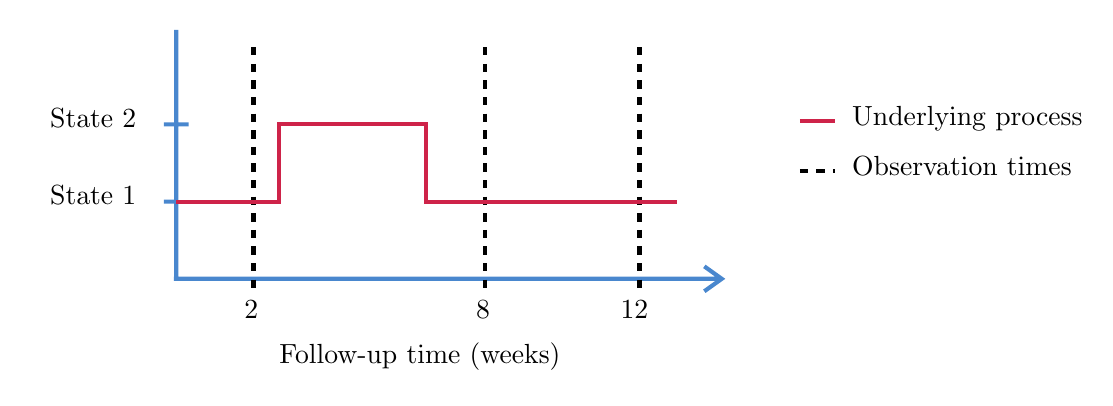
\begin{tikzpicture}[x=0.9pt,y=0.9pt,yscale=-1,xscale=1]
        \path (20,250); %set diagram left start at 0, and has height of 200

        %Shape: Axis 2D [id:dp048941842347560494] 
        \draw [color={rgb, 255:red, 73; green, 135; blue, 206 }, draw opacity=1 ][line width=1.5][-]
        % axes
        (78.67,210.33) -- (298.67,210.33)
        (79.67,110.33) -- (79.67,210.33)

        % arrow
        (291.67,205.33) -- (298.67,210.33) -- (291.67,215.33)

        % axis ticks
        (74.67,179.33) -- (79.67,179.33)
        (74.67,148.33) -- (84.67,148.33);
        \draw;

        \draw [color={rgb, 255:red, 0; green, 0; blue, 0 }, draw opacity=1][line width=1.5][-][dashed]
        (110.67,117.33) -- (110.67,214.33)
        %(141.67,117.33) -- (141.67,214.33)
        %(172.67,117.33) -- (172.67,214.33)
        (203.67,117.33) -- (203.67,214.33)
        %(234.67,117.33) -- (234.67,214.33)
        (265.67,117.33) -- (265.67,214.33)
        (330, 167) -- (344, 167);
        \draw;

        \draw [color={rgb, 255:red, 206; green, 35; blue, 73 }, draw opacity=1 ][line width=1.5][-]

        (79.67,179.33) -- (121.67,179.33)
        (120.85,179) -- (120.85,147.5)
        (120.67,148.33) -- (180.67,148.33)
        (179.85,148.5) -- (179.85,180.15)
        (180.67,179.33) -- (280.67,179.33)
        (330, 147) -- (344, 147);
        \draw;

        %\draw [-] (0,100) node [anchor=north west][inner sep=0.75pt] [align=left] {\textsf{B}};
        \draw [-] (28,172) node [anchor=north west][inner sep=0.75pt] [align=left] {State 1};
        \draw [-] (28,141) node [anchor=north west][inner sep=0.75pt] [align=left] {State 2};
        \draw [-] (106,218) node [anchor=north west][inner sep=0.75pt] [align=left] {2};
        %\draw [-] (137,218) node [anchor=north west][inner sep=0.75pt] [align=left] {4};
        %\draw [-] (168,218) node [anchor=north west][inner sep=0.75pt] [align=left] {6};
        \draw [-] (199,218) node [anchor=north west][inner sep=0.75pt] [align=left] {8};
        %\draw [-] (226,218) node [anchor=north west][inner sep=0.75pt] [align=left] {10};
        \draw [-] (257,218) node [anchor=north west][inner sep=0.75pt] [align=left] {12};
        \draw [-] (120,235) node [anchor=north west][inner sep=0.75pt] [align=left] {Follow-up time (weeks)};

        \draw [-] (350,140) node [anchor=north west][inner sep=0.75pt] [align=left] {Underlying process};
        \draw [-] (350,160) node [anchor=north west][inner sep=0.75pt] [align=left] {Observation times};

    \end{tikzpicture}
    \caption[Example of intermittently-observed data with missed observations for an underlying process]{Example of intermittently-observed data with missed observations for an underlying process.}\label{fig:intermittent-missing}
\end{figure}